\section{Introduction}
\label{sec:intro}

% %!TEX root = ../../main.tex
\begin{figure}[t]
    \centering 
    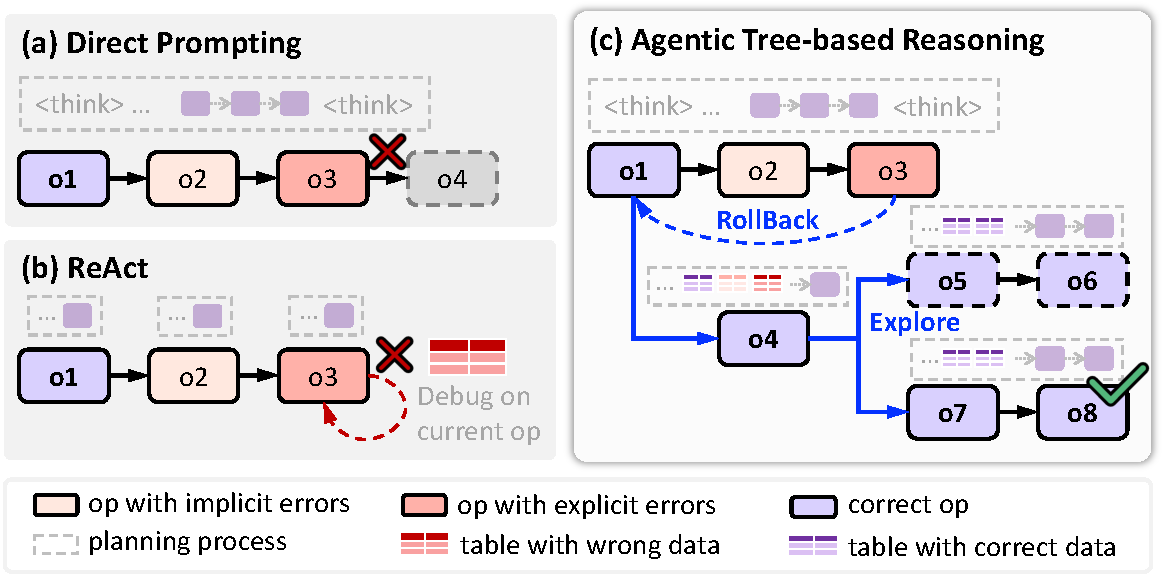
\includegraphics[width=0.99\columnwidth]{figures/fig/prompting_methods.pdf}
    % \vspace{-1em}
    \caption{Comparison of Different Inference Engine.
    }
    \label{fig:prompting_methods}
    % \vspace{-1em}
\end{figure}
%!TEX root = ../../main.tex
\begin{figure*}[!t]
    \centering 
    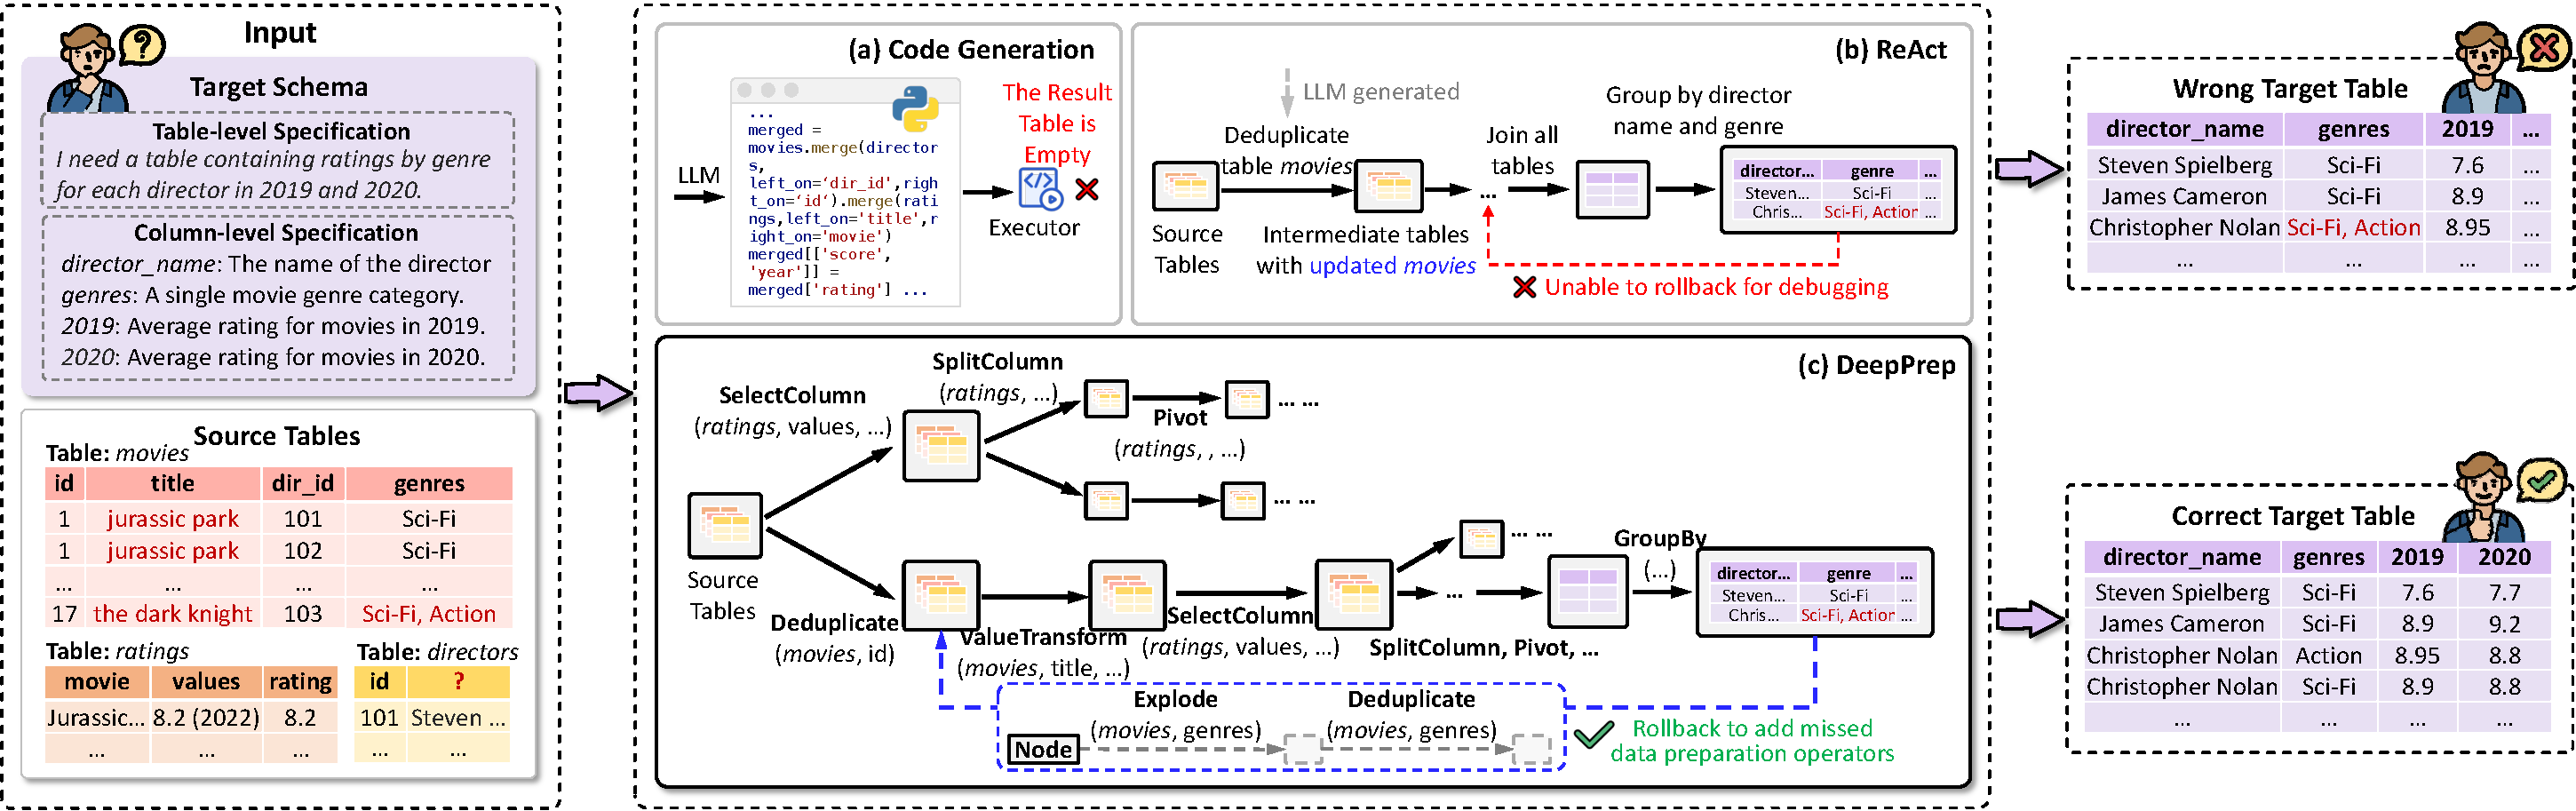
\includegraphics[width=0.95\textwidth]{figures/fig/introduction_example.pdf}
    \vspace{-1em}
    \caption{An illustrative example highlighting the core idea of \sys.
(a) Code generation makes decisions without grounding in intermediate execution results.
(b) ReAct-style approaches follow linear reasoning with limited ability to revise earlier decisions.
(c) \sys applies a tree-based structured exploration, which enables backtracking to resolve non-local errors.
    }
    \label{fig:introduction_example}
    \vspace{-1em}
\end{figure*}

Tabular Data Preparation (DP), the process of transforming raw tables into analysis-ready formats, remains the bottleneck of data science, often consuming 60-80\% of analysis time~\cite{dasu2003exploratory}.
Traditional tools~\cite{barowy2015flashrelate, singh2016blinkfill, he2018transform, gulwani2012spreadsheet, jin2017foofah, heer2015predictive} attempted to automate this process through program-by-example methods. However, these approaches suffer from rigid input-output constraints and lack the flexibility to understand high-level user intent, making them difficult to scale to complex, ambiguous real-world tasks. 

Large Language Models (LLMs) bring opportunity for Natural Language (NL) \nlwhat DP due to its capabilities of NL understanding and reasoning. 
CodeGen~\cite{sapkota2025vibe} interactively generates and execute code (\eg Python program) for specific DP requirement. While flexible, generating raw code for complex, recurring operations is often error-prone compared to standardized operators. Moreover, the uncontrollable granularity of environment interaction makes it difficult to localize errors during debugging. 

\stitle{Operator-Assisted Data Preparation.}
To enhance controllability and stability, recent frameworks (\eg AutoPrep~\cite{fan2024autoprep}) restrict the LLM to generate a sequence of predefined operators. 
% Typically, an end2end data preparation task involves xxx operators in sequence\fmh{cite paper}, and even minor parameter inconsistencies can lead to the failure of the operator's execution due to data inconsistency. 
Previous widely used ReAct framework generates the operator step by step based on the historical execution results. However, 
where the model observes the execution result of step $t-1$ before generating the operator in step $t$, may performs poor in our task.\fmh{cite MCTS paper.}

% Direct Prompting first generates a complete transformation plan and generates the entire chain in a single pass. However, the generated chain is usually in low quality without the signals of intermediate execution results. (2) ReAct framework solves this limitation by adopting step-by-step reasoning, where the model observes the execution result of step $t-1$ before generating the operator in step $t$.

However, we identify fundamental limitations in these linear frameworks.
For Direct Prompting in Figure~\ref{fig:prompting_methods}(a), the system rigidly adheres to a single pre-planned trajectory, failing to explore alternative transformation strategies. Moreover, without access to intermediate execution results, the model operates blindly, making it prone to hallucinating invalid operators or parameters that do not align with the actual data state.
Even for Execution-Aware CoT in Figure~\ref{fig:prompting_methods}(b), which incorporates feedback, the reasoning remains constrained by the \textbf{Markovian Restriction}.
As shown in the figure, when the agent encounters a failure at \texttt{Op3}, it treats the current erroneous state as the fixed starting point for the next step. Constrained by the linear nature, the agent cannot revisit previous decisions; it attempts to patch the error by appending new operators, effectively treating the historical trajectory as immutable.
However, the root cause actually lies in a structural misstep taken earlier (the incorrect \texttt{Op2}). Lacking the mechanism to backtrack and revise that foundational decision, the linear agent is unable to "jump back" to correct \texttt{Op2}, effectively becoming trapped in a local optimum.

\stitle{The Need for Tree-Based Reasoning.}
To overcome the limitation of linear reasoning, it is necessary to introduce a Tree-Based Reasoning Framework. Unlike linear chains that are committed to a single path, a tree structure maintains multiple partial solutions, enabling both broad exploration and strategic backtracking. As shown in Figure~\ref{fig:prompting_methods}(c), when the system encounters a dead-end at \texttt{Op3}, it is not forced to patch the error locally. Instead, it can perform \textit{RollBack} to a stable previous state (\eg after \texttt{Op1}) and \textit{Explore} a completely new branch (starting with \texttt{Op4}). This mechanism effectively breaks the Markovian restriction, allowing the agent to fix early structural errors and navigate the complex search space of DP more robustly.

\begin{example}
Figure~\ref{fig:introduction_example} illustrates a representative DP task: transforming three raw tables (\texttt{movies}, \texttt{ratings}, \texttt{directors}) into a specific analytical report.
Accomplishing this requires two advanced capabilities grounded in \textit{real-time execution feedback}:

% \noindent(1) \textbf{Execution-Guided Exploration.} 
{\em (a) {Execution-Guided Exploration.}}
The optimal transformation path is often ambiguous. As shown in Step 2, the agent does not blindly guess; it spawns parallel branches and evaluates their \textit{actual execution outcomes}. By observing that the \texttt{ExeCode} branch results in an execution failure while the \texttt{SplitColumn} path produces a valid intermediate table, the system can confidently prune the erroneous branch and proceed with the correct strategy. 
In comparison, Direct Prompting rigidly generate to a single linear plan without verifying intermediate states, leading to irreversible failure if the chosen operator (\eg \texttt{ExeCode}) crashes.

{\em (b) {Feedback-Driven Rollback.}}
Complex errors often stem from early structural omissions. In Step 3, \textit{inspection of the intermediate table state} reveals a semantic violation: the \texttt{genres} column still contains combined strings (\eg ``Sci-Fi, Action'') despite the schema requirement. This execution feedback enables the agent to diagnose the root cause, triggering a rollback to the pre-join state to insert an \texttt{Explode} operator.
While for ReAct method, it is restricted to modifying only the current step. For example, it would be trapped trying to patch the already-joined table, unable to backtrack to the pre-join state where the omission (Explode and Deduplicate operations) occurred.

\end{example}

However, a straightforward implementation of tree-based reasoning, Monte Carlo Tree Search (MCTS)~\cite{li2025alphasql}, faces significant challenges in this domain:

(1) Inaccurate Heuristic Selection. In the \textit{Selection} phase, MCTS relies on scalar metrics (\eg UCT scores) to select correct nodes to rollback to previous correct status, which is demonstrated to be inaccurate to rollback to a correct node when occurring an obviously wrong operator.

(2) Isolated Expansion. In the \textit{Expansion} phase, standard MCTS expands nodes based solely on the current path's history. It suffers from state isolation: when expanding a new branch, the model is blind to the failures of sibling branches. Consequently, it cannot "learn from mistakes" made elsewhere in the tree, leading to redundant retrials of invalid logic that has already been proven wrong in parallel attempts. Consider the cases in Figure~\ref{fig:introduction_example}, even the method has generated wrong branch consisting of the operator AddColumn and CodeGen, it still may generate such wrong operators again when expand from the operator SplitColumn.

\stitle{Proposed Method: Agentic Tree-Based Reasoning.}
To transcend these limitations, we propose an {Agentic Tree-Search Algorithm}. Unlike MCTS, which treats the tree as a set of isolated statistics, our agent perceives the entire tree state which includes visited nodes, execution feedback, and error logs as a global context. The agent iteratively interacts with the tree through four defined actions: (i) The agent uses <plan> to analyze the current global tree structure and execution feedback. It generates a natural language rationale to determine the next strategic move. (ii) Based on the plan, the agent selects any node in the current tree and appends a new operator chain to it with <expand>. (iii) The system executes the newly added chain, updating the tree with the resulting data tables or error messages by <execute>. (iv) The agent finally utilize <solution> to conclude the search by selecting a valid root-to-leaf path as the final answer.

It fundamentally resolves the bottlenecks of standard tree search:

\textbf{(1) Semantic Selection vs. Heuristics.}
Instead of relying on opaque numerical scores which is commonly used in UCT selection in MCTS, our \texttt{<plan} action leverages the LLM's semantic reasoning to decide where to backtrack. The agent can diagnose \textit{why} a branch failed (\eg "logic error" vs. "syntax error") and intelligently select the most promising ancestor node for correction, significantly improving search efficiency.

\textbf{(2) Global Context Awareness vs. Isolation.}
By maintaining the entire tree as the state space, the \texttt{<expand} action breaks the state isolation in MCTS when expanding new branches. The agent learns from the collective trial-and-error history. For instance, if the agent observes that a Regex approach failed in a previous branch, it will explicitly avoid generating similar logic in the new branch, effectively pruning the search space based on cross-branch history.

\stitle{Optimization via Systematic Training.}
To fully unleash the potential of our agentic framework, we introduce a systematic training pipeline that addresses the scarcity of high-quality supervision and the difficulty of credit assignment in long-chain reasoning.
First, to overcome the lack of ground truth for intermediate transformation steps, we propose a Bi-Directional Full-Chain Supervision Synthesis method (Section~\ref{sec:data_synthesis}). By combining backward operation-guided inverse synthesis with forward multi-agent translation, we generate a massive dataset of verifiable transformation trajectories.
Next, we implement a Curriculum-based SFT strategy (Section~\ref{sec:agentic_training_framework}) to address the cold-start problem, progressively guiding the model from mastering atomic operators to orchestrating complex tree-based searches.
Finally, to resolve the sparse reward issue inherent in complex reasoning tasks~\cite{shi2025mutual}, we design a Hybrid Reward mechanism within a Multiturn Reinforcement Learning framework. By integrating execution outcomes, partial table matching, and semantic process evaluation, this approach provides dense feedback, enabling the agent to learn robust exploration and rollback strategies.

\stitle{Contributions.}
In summary, our contributions are as follows:

(1) We identify the \textit{Markovian Restriction} in existing linear DP agents and propose an Agentic Tree-Based Reasoning Framework. This framework treats the entire exploration history as a global state, enabling semantic backtracking and cross-branch learning to escape local optima.

(2) We develop a Bi-Directional Data Synthesis pipeline that generates high-quality, fully supervised training data. By combining forward reasoning with inverse operation synthesis, we ensure both the diversity of data quality issues and the correctness of the ground-truth repair sequences.

(3) We propose a Multi-Stage Policy Learning scheme featuring a Hybrid Reward mechanism. This approach effectively solves the credit assignment problem in long-horizon tasks, allowing the model to jointly optimize its planning, expansion, and execution capabilities.

(4) Extensive experiments demonstrate that our method significantly outperforms state-of-the-art baselines in handling complex, ambiguous real-world DP tasks.
